So far \textit{archetype} has been used synonymously with \textit{simplex vertex}, and surely simplex vertices can be considered archetypes - but archetypes are not necessarily simplex vertices. Figure \ref{fig:AA} gives two examples of archetypes in clusters of simulated points, and shows that archetypes are in fact just the intuitive "corner-points" of any point cloud.
The method for inferring these corner-points is called archetypal analysis (AA). It was introduced by Adele Cutler and Leo Breiman in 1994 and developed as an unsupervised learning method for clustering data that is not well-separated\mcite{cutler1994a}. The central idea it to derive a set of archetypes from which all points can be approximated as linear combinations. Below is given a brief introduction to the method.

\subparagraph{The AA factorization problem}
AA solves the following matrix factorization problem. Consider a data matrix $\matr{X} = [\matr{x}_1, \matr{x}_2, ..., \matr{x}_n] \in \mathbb{R}^{m \times n}$. The task of AA is to estimate the two factor matrices $\matr{S} \in \mathbb{R}^{k \times n}$  and $\matr{C} \in \mathbb{R}^{n \times k}$ such as to satisfy the following equation with minimal approximation:

\begin{equation}
	\matr{X} \approx \matr{AS} = \matr{XCS}
	\label{eq:AA}
\end{equation}

The number of archetypes is controlled by $k$ and can be chosen by the analyst, while the archetypes themselves are column vectors in $\matr{A} \in \mathbb{R}^{m \times k}$. $\matr{C}$ and $\matr{S}$ are column stochastic matrices subject to $|\matr{c}_j|_1 = |\matr{s}_i|_1 = 1$. Columns in $\matr{C}$ give the coefficients of each archetype as a linear combination of the data points, and reversely $\matr{S}$ give the coefficients of each data point as an approximate linear combination of the archetypes. This leads to the property that archetypes may be derived from data points as $\matr{A} = \matr{XC}$ and data points approximated from archetypes as $\matr{X} \approx \matr{AS}$. This introduces symmetry into the matrix factorization problem consistent with the following statement: \textit{archetypes are convex combinations of the data points and data points are approximated by convex combinations of archetypes}. $\matr{C}$ and $\matr{S}$ are derived by minimizing the residual sum of squares ($RSS$):
\begin{equation}
	RSS = \|\matr{X} - \matr{XCS}\|_F^2
	\label{eq:AALossFunction}
\end{equation}
subject to $|\matr{c}_j|_1 = 1\,\, \forall \,\, j \in \{0, ..., k\}$ and $|\matr{s}_i|_1 = 1 \,\, \forall \,\, i \in \{0, ..., n\}$, where $\| \cdot \|_F$ is the Frobenius norm. Furthermore, AA imposes the constraint that all coefficients of $\matr{C}$ and $\matr{S}$ are greater or equal to zero. Note that $RSS$ goes to zero in the limit $\matr{AS} \rightarrow \matr{X}$ where the data points can be  reconstructed exactly as convex combinations of the archetypes. It can be shown that Equation \eqref{eq:AALossFunction} is non-convex, and that the optimization problem has no closed form solution\mcite{cutler1994a}, yielding numerical methods necessary for solving the problem.

\begin{figure}
	\centering
	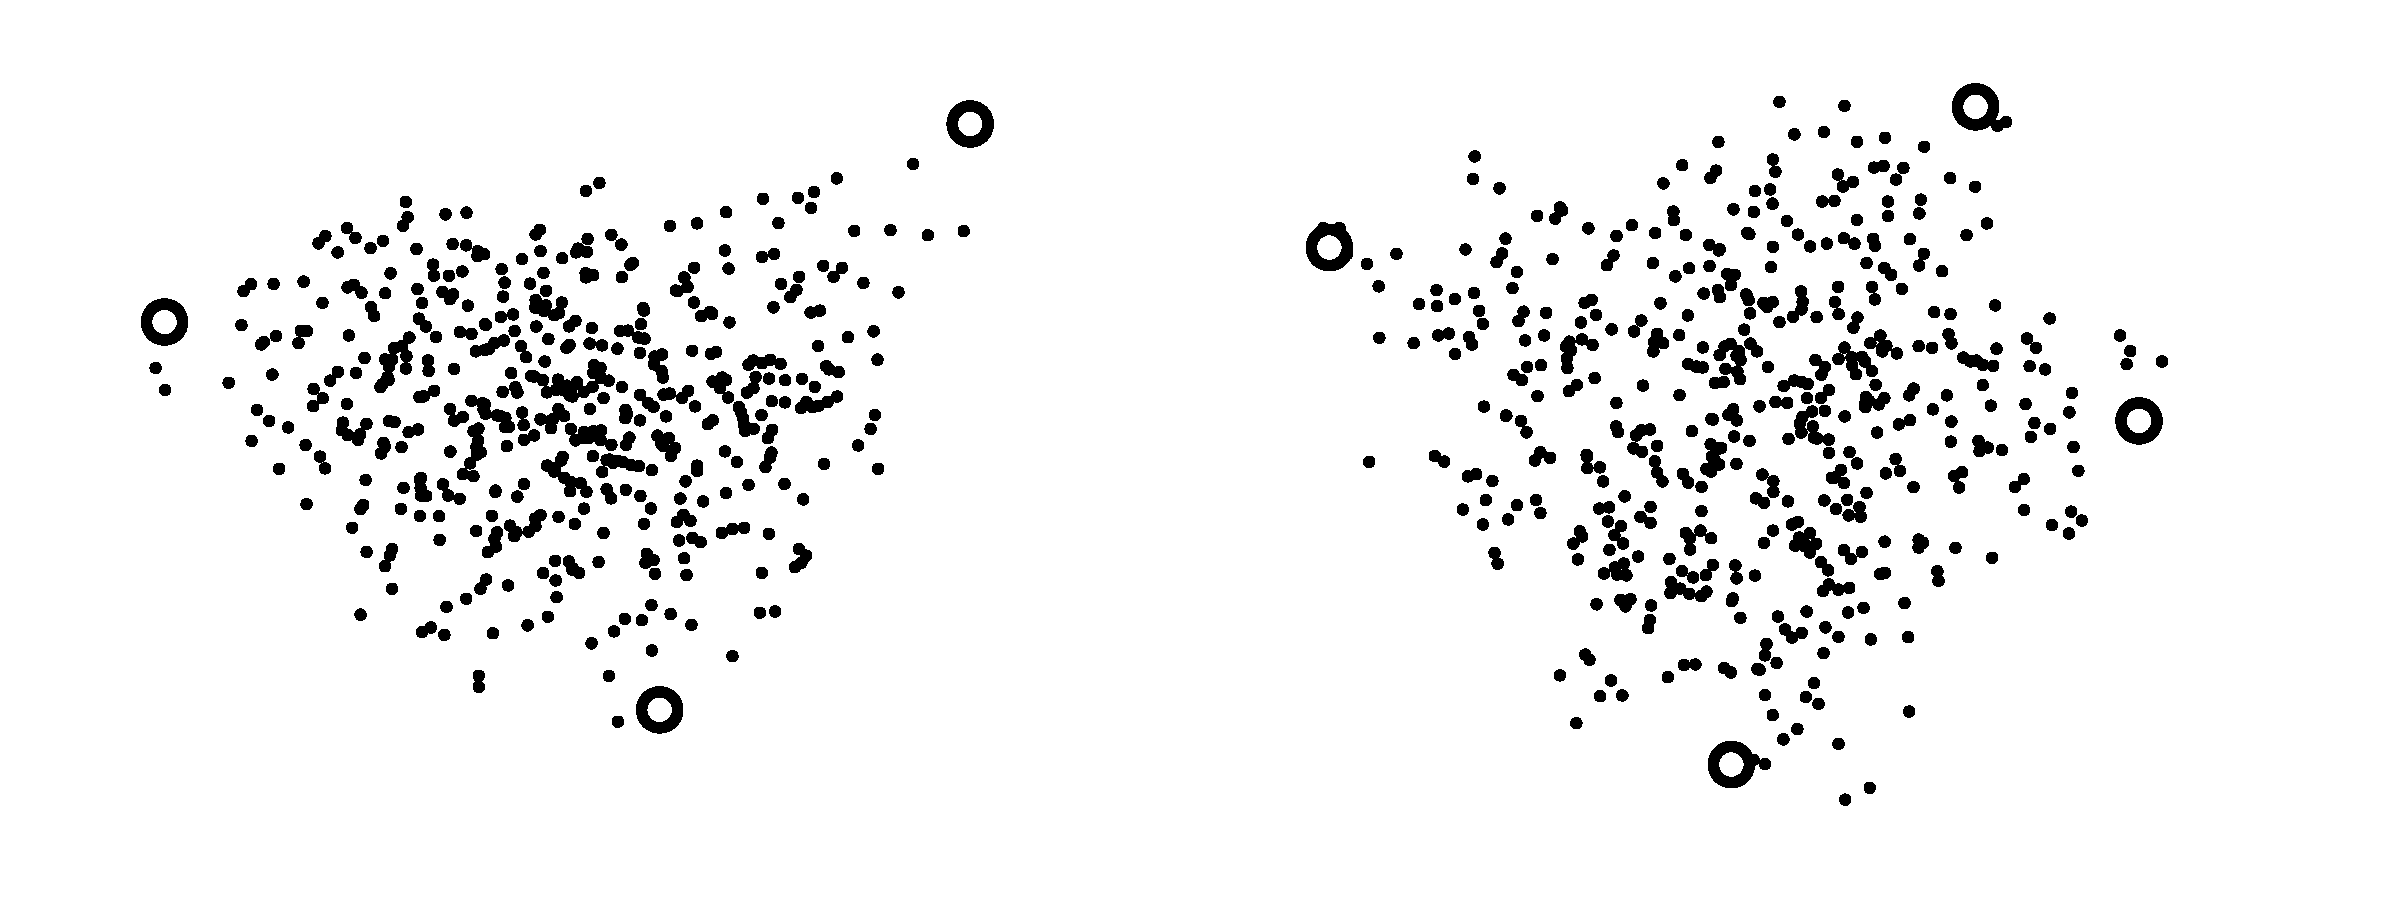
\includegraphics[width=1\linewidth]{figures/AA}
	\caption{\label{fig:AA}Two generic examples of archetypes in multidimensional data. Hollow circles represent the archetypes which are typically located in \textit{corner}-like regions of the data.}
\end{figure}

\subparagraph*{Numerical methods for estimation of archetypes}
Cutler et. al. solved the AA problem using an alternating optimization approach. Starting from a random initialization of $\matr{S}$ the method alternates between finding the best $\matr{C}$ for an $\matr{S}$ and finding the best $\matr{S}$ for a $\matr{C}$, for as necessary until the reduction in $RSS$ is sufficiently small. Each iteration requires solving several convex least squares problems and convergence is slow for many points in high dimensions because the number of points on the convex hull increases exponentially (see Figure \ref{fig:convexHullCurseOfDimensionality}.a. Recent work due to M\o rup and Hansen introduces an effective initialization procedure and a projected gradient approach to solving the AA matrix factorization problem, which however reduces the computation time by limiting the number of points on the convex hull that can constitute solutions to the optimization problem\mcite{morup2012archetypal}. It furthermore allows the analyst to compute archetypes with \texit{slack} such that they may fall outside of the convex hull, diminishing the problem illustrated in Figure \ref{fig:convexHullCurseOfDimensionality}.b.


\subparagraph*{Available implementations}
A number of implementations of AA are available across different software languages. Morup et. al. gives an implementation of their proposed projected gradient version of AA\mcite{morup2012archetypal} which has furthermore been translated into a Python package, by this author, available on the Python Package Index (PyPI). The Python package PyMF also gives an implementation of the, however, slightly slower alternating optimization version of AA\mcite{pymf}. Finally, there is an implementation in R that also uses the traditional approach\mcite{eugster2009spider}.

\subparagraph*{Alternative methods}
As far as the ParTI principle is concerned the only requirements of archetypes is that they constitute the geometrical corners of the dataset. As such other methods for computing archetypes are just as valid as AA. Four alternative methods estimate archetypes using minimal volume simplex and spectral unmixing methods using different approaches\mcite{bioucas2009variable, li2008minimum, chan2009convex, bioucas2009variable}. It is, however, not within the scope of this thesis to further discuss any of these methods.